%
% aj - for a future version of this paper - I think, we should extract the
%       requirements of KV-stores as they are required by VMS, expose
%       them as part of the discussion here and provide a summary table
%       either here or in RW that shows which existing KVS has what
%       feature we require (some do, others don't.)
%
\section{KV-store Model}
\label{sec:kv_model}

In this section, we provide background information about KV-store
internals that serve us in the remainder of this paper.  We abstract
from any particular store, focusing on the main concepts, grounding
them in existing systems such as~\cite{chang:bigtable,
  decandia:dynamo, cooper:pnuts, george:hbase, hewitt:cassandra}. 
The section is organized as follows: we discuss the design of the 
KV-Store and its components; we depict the processing of 
a client operation through the KV-store architecture; we define a common data 
model for KV-stores; and we identify extension points that will later
serve to connect KV-store to VMS.


  
  

\subsection{Design}


Some KV-stores are based on a master-slave architecture, i.e. HBase;
other KV-stores run without a master, i.e. Cassandra (a leader 
is elected to perform tasks controlling the KV-store). 
In both cases a \textit{node} represents the unit of scalability -- 
as arbitrary instances can be spawned in the network (see 
Figure~\ref{fig:kv_model}). The node persists the actual data.  But in
contrast to a traditional SQL-database, a node manages only part of the 
overall data (and request load). As load grows in the KV-store, more 
nodes can be added to the system; likewise, nodes can be removed as load 
declines. The KV-store will automatically adapt to the new situation and 
integrate, respectively drop the resource. KV-stores differ in how they 
accommodate;  they also differ in how they perform load balancing and 
recovery (in face of node crashes). However, with regard to nodes, we can 
describe a set of universal events that occur in every KV-store 
(cf. Table~\ref{tab:kvs_a_events}).


A \textit{file system} builds the persistence layer of a node in a
KV-store. For example, HBase stores its files in the Hadoop distributed
file system (HDFS). Cassandra does not employ a distributed file system.  
Instead, its nodes access the local file system to store commit log and 
table files. Nevertheless, Cassandra also relies on its own replication 
mechanism. Replication enables the KV-store to keep its files available 
and safe in the presence of failures. If a node (and even its local file 
system) crashes, a copy on one of the replica nodes will be used to restore
the data.  

A \textit{table} in a KV-store does not follow a fixed schema. It stores 
a set of table records called \textit{rows}. A row is uniquely identified by a
\textit{row key}. A row holds a variable number of \textit{columns}
(i.e., a set of column-value pairs). Columns can be further
grouped into \textit{column families}. Column families provide fast
sequential access to a subset of columns. They are determined when a
table is created and affect the way the KV-store organizes its table
files.\\ 
\textit{Key ranges} serve to partition a table into multiple
parts that can be distribute over multiple nodes.  Key ranges are
defined as an interval with a start and an end row key.  PNUTS refers
to this partitioning mechanisms as tablets, while HBase
refers to key ranges as regions. Multiple regions can be
assigned to a node, often referred to as a region server. 
In general, a KV-store can split and move key ranges between nodes to 
balance system load or to achieve a uniform distribution of data. With
regard to key ranges, we can also describe a set of universal events 
(cf. Table~\ref{tab:kvs_a_events}).

%
%Cassandra defines a table as a key space. A node only manages a single
%key space, which may overlap with spaces of neighboring nodes.
%
%In these systems, key ranges can be either managed automatically or
%predefined manually.

\begin{figure} 
	\centering 
	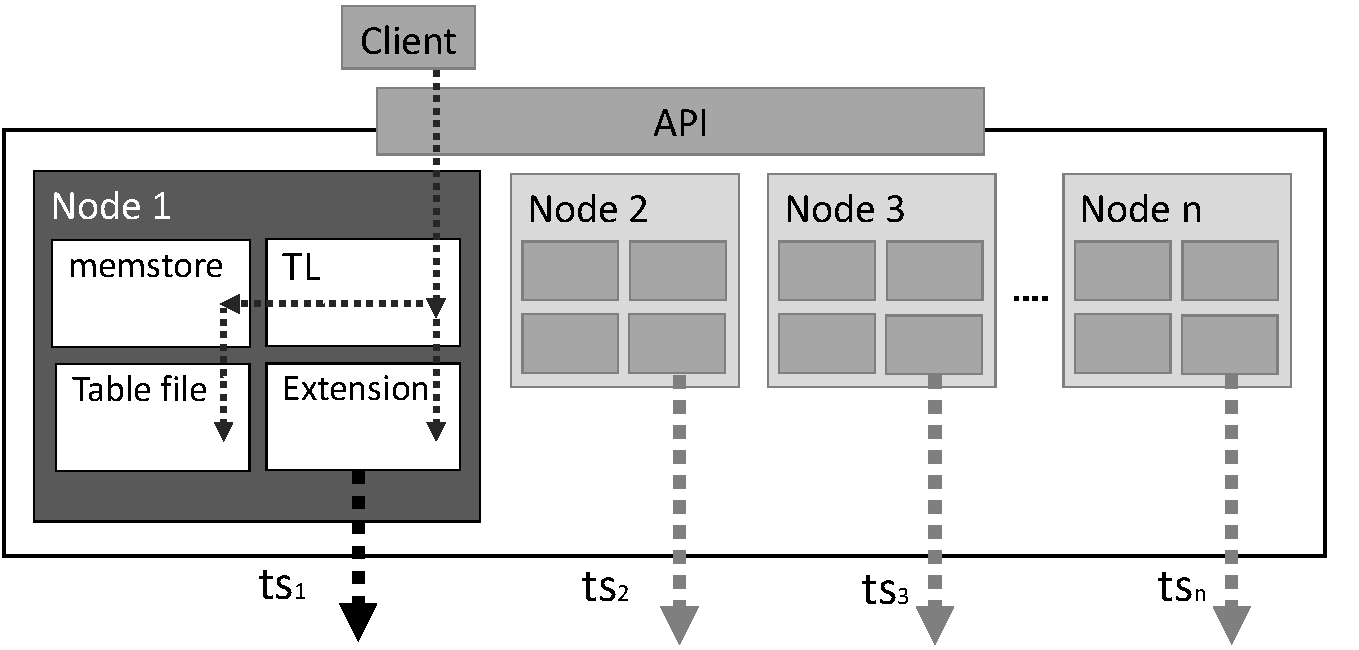
\includegraphics[width=\linewidth]{figures/KVModel} 
	\caption{KV-model} 
	\label{fig:kv_model} 
\end{figure} 

\subsection{Operation processing}


The KV-store API allows for three simple \textit{client operations}: put, which
inserts a record; get, which retrieves a record; and delete, which 
removes a record\footnote{There are additional methods, e.g. a range scan. However, none of them extends beyond repeated single 
row access; none of them offers expressive semantics.}. Now, we describe the path 
of a client operation, manipulating the data via put or delete statement, through 
the KV-store architecture.


The system routes the client request to the serving
node. When updating a table record, clients only access a single node,
i.e., the one that serves the accessed record. This reduces access
time and distributes client requests among all system nodes. For
example, HBase routes client requests from a root node down to the
serving node in a hierarchical manner. Cassandra, on the other hand,
lets the clients connect to an arbitrary node. This node forwards the
request to the serving node. In both cases, the client eventually
transmits its request to the serving node.

Every node maintains a \textit{transaction log} (TL). In HBase it is
called write-ahead log, whereas Cassandra refers to it as
commit log. When a client operation arrives, it is first written
into the transaction log of the node (cf. Figure~\ref{fig:kv_model}). From 
then on, the operation is persisted durably -- as the TL is stored and 
replicated at the file system that we discussed before.

Then, the operation is inserted into a
\textit{memstore}.  Memstores are volatile; upon a node crash, they
can be recovered from the TL, which contains the operation sequence a
node saw over time.   During recovery, this sequence is replayed from 
the log. Once a memstore exceeds a set capacity, it is flushed to disk.  
Continuous flushes produce a set of table files, which are periodically 
merged by a compaction process. After a flush, the corresponding entries 
in the TL can be purged. 


\subsection{Data model}

The data model of a KV-store differs from that of a
relational DBMS.  We describe a model that is representative for
today's KV-stores. The model serves throughout the paper to help
specify views and view update programs. Typically, KV-stores do not
required fixed data schemas, but rather accommodate dynamic schema
changes.

Thus, we formalize the data model of a KV-store as a map of key-value 
pairs $\{\langle k_1, v_1\rangle,..,\langle k_n,v_n\rangle\}$ described 
by a function $f:K \rightarrow V$. Systems like BigTable, HBase and 
Cassandra established data models that are multi-dimensional maps 
storing a row together with a variable number of columns per row. For 
example, the 2-dimensional case creates a structure 
$\{\langle(k_1,c_1),v_{1,1}\rangle,\langle (k_n,c_n) ,v_{n,n}\rangle\}$ 
with a composite key $(k_n,c_n)$ that maps to a value $v_{n,n}$ 
described by $f:(K,C)\rightarrow V$. In the 3-dimensional case, another 
parameter, a timestamp, for example, is added to the key, which may 
serve versioning purposes. For the intentions in this paper, the 
2-dimensional model suffices.\footnote{Our approach also works with the 
1-dimensional case, which is representative for simple key-blob stores. 
We use the 2-dimensional case here, as it is more expressive.} 

We denote a table by $A = (K, F)$, where $K$ represents the row key and 
$F$ a \textit{column family}. Column families are defined when a table 
is created. They are used in practice to group and access sets of 
column-value pairs. In terms of our data model, column families are 
optional. They can be dynamically assigned as the row is created. Let a 
base table row $a \in A$ be defined as $a=(k,\{\langle 
c_1,v_1\rangle..\langle c_n,v_n\rangle\})$. In this notation, the row 
key $k$ comes first, followed by a set of column-value pairs $\{\langle 
c_1,v_1\rangle..\langle c_n,v_n\rangle\}$ belonging to 
the column family; this more closely resembles a database row and is 
used throughout the remainder of this paper. When using multiple column 
families, we define the table as $A = (K, F_1,...F_n)$. Then the 
assignment of a column-value set to a column family $F_x$ is denoted by 
$\{..\}_x$. The corresponding row would be defined as $a=(k, \{\langle 
c_1,v_1\rangle..\langle c_i, v_i\rangle\}_1..., \{\langle 
c_{i+1},v_{i+1}\rangle.. \langle c_n,v_n\rangle\}_n)$. 



\subsection{Extension points}
Extension points are interfaces that can be used to interact with the
KV-store. Since our VMS only reacts to the KV-store -- as we don't
interfere with its data processing -- we are interested in events
exclusively. There are two different kinds of events our VMS needs 
to react to: Administrative events and data events.

\subsubsection{Administrative events}

These events (Table~\ref{tab:kvs_a_events}) occur during a state change in the KV-stores 
infrastructure, e.g. a new node is added to the KV-store (and starts 
processing client operations).  The KV-store 
implementations provide different ways to react to administrative 
events. HBase lets developers use various kinds of Coprocessors. The 
latter represent little pieces of code that can be deployed on the 
KV-store nodes. Thus, we can modify a Coprocessor to notify our VMS, as 
soon as the new node is added. The VMS reacts accordingly and allocates 
resources to maintain the view tables that depend on the new node. 



\begin{table}
\rowcolors{2}{gray!10}{gray!30}
\setlength{\belowrulesep}{0pt}
\setlength{\aboverulesep}{0pt}
\setlength\extrarowheight{2pt}
\begin{center}
\begin{tabular}{l l l}
\toprule
Component & Event & Method \\
\midrule
Node & added & \textit{onNodeAdded()}  \\
 & removed & \textit{onNodeRemoved()}    \\
Key-range & opened   & \textit{onKeyRangeOpened()}\\
 & closed & \textit{onKeyRangeClosed()} \\
 & split & \textit{onKeyRangeSplit()} \\
  & moved & \textit{onKeyRangeMoved()} \\
%Transaction log & replay & \textit{onTLReplay()}\\
% & purge & \textit{onTLpurge()} \\ 
\bottomrule 
\end{tabular}
\caption{Administrative events}
\label{tab:kvs_a_events}
\end{center}
\end{table}

\subsubsection{Data events}


When the client updates a base table (put, get, delete) a data event
occurs. The view tables become stale and the VMS needs to update them
correspondingly. We identified three different methods to stream updates
on base data from KV-store: (1) Access KV-API, 
(2) intercept KV-store operations (e.g. Coprocessors), (3) read the 
transaction log. Method (1) is not feasible, because we do not receive 
consistent snap-shots of the data -- as records may change during the 
scanning process. Moreover, we create a lot of performance overhead. 
Method (2) is promising with regard to freshness of the view (as it is 
synchronous), but only suitable if the number of maintained views is 
small. As it grows large, operations of the KV-store are delayed to a 
great extent.
 
Method (3) as opposed to (2), has several benefits: (i) Reading the TL 
is asynchronous. It neither interferes nor imposes additional load on the 
KV-store processing. \footnote{Our experiment results showed that the 
penalty of reading from the file system 
are far smaller than intercepting events.}(ii) Maintaining numerous views at once means 
that every base table operation generates multiple view updates. Using the
transaction log, we decouple the view update from the client operation  
 (iii) Operations in the TL are durably persisted and can be recovered, 
 not only by the KV-store, but also by VMS. (iv) The transaction log contains
 client operations, not table rows, which is fine for incremental and 
 deferred view processing.

The KV-store writes operations, that is client requests, to the TL,
but not entire table rows.  In contrast, a table row stores the row
state, which may result from multiple client requests.  Then, an 
operation $t \in T$ can easily be defined over table row $a \in A$,
with $T = type(A)$  and $type \in \{put, delete\}$. A put operation in
the transaction log is denoted as $t=put (k, \{\langle c_1,v_1\rangle..\langle
c_n,v_n\rangle\})$. A put inserts or updates the column values at the
specified row key. A delete operation $t \in T$ is defined as
$t=delete (k, \{\langle c_1,\emptyset\rangle..\langle
c_n,\emptyset\rangle\})$.  Note that we are leaving the values 
empty; the client just specifies the row key and columns that are to
be deleted. A stream -- respectively, the output of one node's transaction log --
is denoted as a sequence of operations $ts \in TS=(T_1,..,T_n)$. Finally, we can
define the complete output of the KV-store as a set of operation 
streams as $ts_1,..ts_n \in TS$. 


%
% aj - above - does a delete w/ columns only delete the column values
%                     or the entire record?
%
